\chapter{Konzept}
\label{chap: Konzept}

\begin{figure}[b]
	\centering
	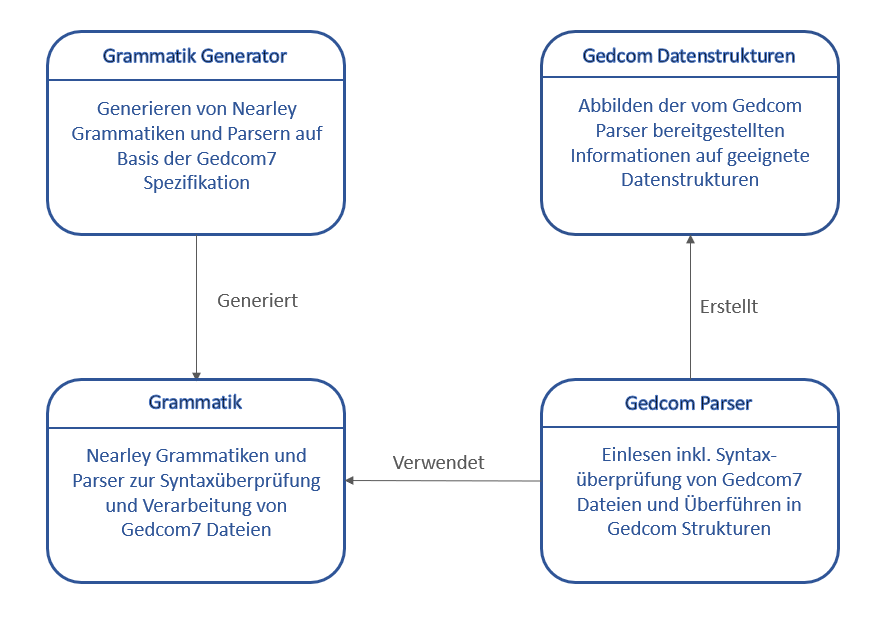
\includegraphics[width=0.85\textwidth]{images/konzept_allgemein.png}
	\caption{Allgemeiner Aufbau}
	\label{fig: Allgemeiner Aufbau}
\end{figure}

Die Bibliothek \textit{gedcom7.js} lässt sich wie in \hyperref[fig: Allgemeiner Aufbau]{Abbildung 4.1} dargestellt in vier logische Teile gliedern. Das zentrale Element ist der \textsc{Gedcom Parser}, mit dem Dateien oder Strings im in Abschnitt \ref{sec: GEDCOM Version 7} vorgestellten Format gedcom7 eingelesen werden und mit Hilfe von \hyperref[sec: Nearley]{\textit{Nearley}} auf Korrektheit der Syntax überprüft werden können. Die dafür zugrundeliegende Grammatik wird mit Hilfe eines \textit{Grammatik Generators} generiert, der die in \cite{GEDCOM} definierte Spezifikation in eine Nearley-konforme Syntax überführt. Die so eingelesenen Informationen werden in Gedcom Datenstrukturen gespeichert, die verändert und erweitert werden und anschließend im Format gedcom7 ausgegeben werden können. In den folgenden Abschnitten werden die vier Teile und das Zusammenspiel dieser in detaillierter Form vorgestellt.

%========================================================================================
% SECTION: GEDCOM GRAMMATIK
%========================================================================================
\section{Gedcom Grammatik}
\label{sec: Konzept - Gedcom Grammatik}
Eine wichtige Anforderung an die Bibliothek \textit{gedcom7.js} ist, dass die Syntax von Dateien oder Strings, die eingelesen werden, gemäß der Gedcom7-Spezifikation überprüfbar sein soll. Da die Gedcom Datenstrukturen veränderbar und erweiterbar sein sollen, ist es wichtig, dass eine Syntaxüberprüfung nach Änderungen auf einfache Weise möglich ist. Umgesetzt wird diese Syntaxüberprüfung mit Hilfe des in \hyperref[sec: Nearley]{Kapitel 2.3} vorgestellten JavaScript-Parser-Toolkits \textit{Nearley}. Mit \textit{Nearley} können auf einfach Weise, menschenlesbare Grammatiken erstellt und zu einem \textit{Nearley-Parser} kompiliert werden. Von großem Vorteil ist dabei, dass Features wie Postprozessoren und die Implementierung eines Lexers unterstützt werden. 

\subsection{Pre- und Postprozessor}
\label{subsec: Konzept - Gedcom Grammatik - Pre- und Postprozessor}
Standardmäßig packt ein \textit{Nearley-Parser} jedes Zeichen, das mit einer Regel übereinstimmt, in ein Array \cite{NearleyDoc}. Bei komplexeren Grammatiken wie der Gedcom7 Spezifikation führt dies dazu, dass sehr viele Arrays ineinander verschachtelt werden, sodass schnell zweistellige Verschatlungsgrade erreicht werden, was ein Weiterarbeiten mit den Ergebnissen erschwert. Mit Hilfe von Postprozessoren können jeder \textit{Nearley Regel} Verarbeitungsanweisungen zugewiesen werden, sodass die Ergebnisse beispielsweise im JSON-Format zurückgegeben werden. Auf diese Weise können die eingelesenen Dateien bereits bei der Syntaxüberprüfung in eine passende Darstellungsform gebracht werden, sodass eine leichte Überführung in die passende Gedcom Datenstruktur möglich ist.

Desweiteren kann ein Lexer verwendet werden, um die Arbeit mit \textit{Nearley} zu optimieren. Ein \textit{Nearley-Parser} teilt die Eingabedaten standardmäßig in einen Strom von einzelnen Zeichen, die sequentiell abgearbeitet werden, was auch als \textit{Scannerless Parsing} bezeichnet wird \cite{NearleyDoc}. Ein Lexer ist eine Art Preprozessor, der die Eingabedaten in größere Einheiten, die sog. \textit{Tokens} zusammenfasst \cite{NearleyDoc}. Auf diese Weise wird der Aufwand beim Parsen verringert und die Interpretation der Eingabedaten fällt oft leichter. Ein einfaches Beispiel hierfür ist eine Regel die einen Zahlenwert erwartet. Ist der Eingabewert beispielsweise "137", würde ein \textit{Nearley-Parser} standardmäßig jede Ziffer einzeln einlesen und im Postprozessor müsste definiert werden, dass die aufeinanderfolgenden Ziffern als ein Zahlenwert interpretiert werden sollen. Mit Hilfe eines Lexers könnte eine einfache Regel definiert werden, die den kompletten Zahlenwert als ein Token vorverarbeitet. Im Rahmen dieser Arbeit wurde der JavaScript Lexer \textit{Moo.js} \cite{MooDoc} verwendet. \textit{Moo.js} zeichnet sich durch seine Geschwindigkeit aus und wird von \textit{Nearley} als Lexer unterstützt.\footnote{Laut den Entwicklern ist Moo.js der schnellste JavaScript-Lexer und $\sim$2-10 mal schneller als herkömmliche Lexer \cite{MooDoc}.} 
\newpage
\subsection{Nearley-Parser für Gedcom7}
\label{subsec: Konzept - Gedcom Grammatik - Nearley-Parser für Gedcom7}
Da sowohl die Gedcom7- als auch die Nearley Syntax auf \hyperref[sec: Nearley]{EBNF-Sprachkonzepten} basieren, lässt sich die Gedcom7 Spezifikation ohne weiteres in eine Nearley Grammatik übersetzten, die dann zu einem Nearley-Parser kompiliert werden kann. Wird diesem Nearley-Parser eine Gedcom7-Datei (.ged) kodiert als UTF-8 Zeichenkette übergeben, erfüllt dieser die folgenden zwei Aufgaben:

\vspace{1em}
\textbf{1. Überprüfung der Gedcom7 Syntax} \vspace{0.35em} \\
Der Nearley-Parser überprüft den übergebenen Gedcom7-String Line für Line, indem er alle Zeichen (bzw. Tokens) sequentiell liest, bis ein End-Of-Line (EOL) Token  gefunden wird. Nach jedem Zeichen das eingelesen wird, überprüft der Parser, welche in der Grammatik definierten Regeln durch das neu eingelesene Zeichen nicht mehr mit der Zeichenkette übereinstimmen und verwirft diese. Wird ein EOL Token gelesen werden die Postprozessoren aller übereinstimmenden Regeln ausgeführt und ein Array mit den Ergebnissen dieser Postprozessoraufrufe als Ergebnis der Line zurückgegeben. Da die Gedcom7 Grammatik nicht mehrdeutig ist, findet der Parser bei korrekter Gedcom7 Syntax immer ein eindeutiges Ergebnis (d.h. beim Erreichen des EOL Tokens ist maximal eine übereinstimmende Regel übrig). Werden bei diesem Prozess alle Regeln der Grammatik ausgeschlossen, bevor ein EOL Token gelesen wird, ist die Syntax des übergebenen Gedcom7-Strings nicht korrekt und das Parsen kann mit einem Syntaxfehler abgebrochen werden. Da die Zeichenkette sequentiell abgearbeitet wird, kann bei auftretendem Fehler genau aufgezeigt werden, welche Line und welches Zeichen fehlerhaft sind.

\vspace{1em}
\textbf{2. Extrahieren der Structure-Informationen} \vspace{0.35em} \\
Eine weitere Aufgabe des Nearley-Parsers ist es, die Structure-Informationen des Gedcom7-Strings zu extrahieren, sodass im nächsten Schritt eine einfache Über-führung in entsprechende Gedcom Datenstrukturen möglich ist. Durch den sequentiellen Aufbau einer Gedcom7 Datei wird eine Structure stets vor ihren Substructures definiert. Da das erste Token jeder Line stets das Level der Line repräsentiert, kann der Nearley-Parser die Abhängigkeiten der Lines zueinander zuordnen und es ist zu jedem Zeitpunkt eindeutig, welcher Superstructure eine Structure zugeordnet werden soll. Folgende Informationen können also durch den Nearley-Parser extrahiert werden: 
\begin{itemize}
	\item \textbf{URI}: Auch wenn bestimtme Structuretypes denselben Tag besitzen, kann aus der Kombination von Level und Tag die eindeutige Gedcom URI bestimmt werden
	\item \textbf{Datentyp}: Sofern ein Payload in der Line vorhanden ist, kann mit Hilfe der URI der Datentyp des Payloads bestimmt werden
	\item \textbf{Superstructure}: Zu jeder Line kann die entsprechende Superstructure angegeben werden, sofern es sich nicht um einen Record (Structure mit Level 0) handelt, die keine Superstructure besitzen
	\item \textbf{Substructures}: Hat eine Sturktur eine oder mehrere Substructures, können diese auf Basis des Levels der Lines bestimmt werden
\end{itemize}

%========================================================================================
% SECTION: GRAMMATIK GENERATOR
%========================================================================================
\section{Grammatik Generator}
\label{sec: Konzept - Grammatik Generator}
% Warum Grammatik Generator -> Anforderung erweiterbar
% Wie umgesetzt? -> JS-Definitionsdateien einlesen 
% Ablauf -> einlesen, grammatik erstellen, kompilieren,
In der Gedcom7 Spezifikation werden 181 Structuretypes verteilt auf 7 Records definiert, die alle in einer Line der Form
\begin{lstlisting}[frame=none]
	Level  D  [Xref  D]  Tag  [D  LineVal]  EOL
\end{lstlisting}
dargestellt werden. Sollen diese Structuretypes in eine Nearley Grammatik überführt werden, muss für jede dieser Structures und jede mögliche Kombination an Substructures eine Regel erstellt werden. Da dies eine sehr repetitive Aufgabe ist und sich die Regeln nur an bestimmten Stellen unterscheiden, lässt sich die Grammatikerstellung durch einen Grammatik Generator automatisieren. Dazu können Definitionsdateien erstellt werden, die die für alle Structuretypes die folgenden Informationen bereithalten: 
\begin{itemize}
	\item \textbf{URI}: Die URI des Structuretypes wird benötigt, um eine Structure eindeutig zuordnen zu können 
	\item \textbf{LineType}: Der LineType gibt an, wie die Line aufgebaut ist - also ob bspw. ein Cross-Reference-Identifier oder ein Payload vorhanden sind
	\item \textbf{Datatype}: Sofern ein Payload in der Line vorhanden ist, kann über den Datatype die Syntax des Payloads ermittelt werden
	\item \textbf{Tag}: Der Tag wird benötigt, um die Line einer Nearley Regeln zuordnen zu können
	\item \textbf{Substructures}: In der Gedcom7 Spezifikation sind für alle Structuretypes alle zulässigen Substructures definiert. Mit dieser Information können alle syntaktisch korrekten Structures in Nearley Regeln abgebildet werden.
	\item \textbf{Level}: Um eine eindeutige Grammatik zu generieren, müssen die Level mit denen ein jeweiliger Structuretype auftreten kann, zwingend mit angegeben werden. Da in der Gedcom7 Spezifikation Tags mehrfach für verschiedene Structuretypes verwendet werden, kann nicht einfach ein generisches Level für die Regeln verwendet werden, das ganzzahlige Werte akzeptiert, da die entstehende Grammatik damit mehrdeutig wäre. Ein Beispiel hierfür sind die Structures \textit{g7:HEAD-DATE} und \textit{g7:DATE-exact} im Gedcom Header. Mit einem generischen Level wären die Regeln für beide Structuretypes identisch mit 
	\begin{lstlisting}[frame=none]
	  Level  D  "DATE"  D  DateExact  EOL
	\end{lstlisting}
	Wird eine solche Line als Substructure eines Header Records von dem Nearley Parser gelesen, kann dieser nicht entscheiden, ob es sich um ein \textit{g7:HEAD-DATE} oder ein \textit{g7:DATE-exact} handelt und würde somit zwei Ergebnisse aufrecht erhalten. Um diese Mehrdeutigkeit zu verhindern, wird das Level in der Definition angegeben. Da die Structure \textit{g7:HEAD-DATE} mit dem Level $+1$ und \textit{g7:DATE-exact} mit Level $+3$ bezogen auf den zugrundeliegenden Header Record vorliegen, können die Lines vom Parser eindeutig unterschieden werden.
\end{itemize}
\newpage
Anhand dieser Informationen kann der Grammatik Generator automatisiert Nearley Regeln formulieren. Diese Regeln können zu einer Grammatik zusammengefasst und anschließend vom Generator zu einem Nearley-Parser kompiliert werden. Anhand des LineTypes kann der Generator den Regeln die passenden Postprozessoren zuweisen, die für das Extrahieren der Structure Informationen zuständig sind. Auf diese Weise kann ein voll funktionaler Nearley-Parser automatisiert generiert werden, der die Gedcom7-Syntax vollständig parsen und alle für die weitere Verarbeitung benötigten Informationen extrahieren kann. 


Ein weiterer großer Vorteil an dieser Automatisierung ist, dass zur Erfüllung der Anforderung der einfachen Erweiterbarkeit der Bibliothek beigetragen wird. Sollte die Grammatik in zukünftigen Projekten erweitert werden, bspw. wenn in einer neuen Version des Gedcom Standards weitere Structuretypes definiert werden, ist dies auf einfache und verständliche Weise durch das Hinzufügen neuer Einträge in die Definitionsdatei des Grammatik Generators möglich. 


Desweiteren bildet der Grammatik Generator ein Fundament für einen wichtigen Use-Case, der in weiterführenden Arbeiten adressiert werden sollte: der Möglichkeit Extensions zu definieren. Die Gedcom7 Spezifikation definiert die wichtigsten Strukturen zur Speicherung genealogischer Informationen - für alle Informationen, die über diese Standardstrukturen hinausgehen, müssen Extensions definiert werden. Da genealogische Informationen sehr vielfältig sein können, sind Extensions ein probates Mittel, dass in vielen Anwendungen genutzt wird. Mit Hilfe des Grammatik Generators kann die Definition von Extensions umgesetzt werden, indem eine Schnittstelle zum Generator entwickelt wird, die dem Benutzer zur Verfügung gestellt wird. Über diese Schnittstelle kann die Definitionsdatei erweitert werden und anschließend die Grammatik neu generiert und kompiliert werden. Auf diese Weise könnte die Bibliothek auf die Anforderung aller Benutzer angepasst werden. 
%========================================================================================
% SECTION: GEDCOM STRUKTUREN
%========================================================================================
\section{Gedcom Datentrukturen}
\label{sec: Konzept - Gedcom Strukturen}
Die zentrale Struktur in einer Gedcom7 Datei ist das sog. \textit{Dataset}. Jedes Dataset muss mit einem Header Structure beginnen, der Metadaten über das gesamte Dataset beinhaltet und dabei u.a. Aussagen über den Ort und Zeitpunkt der Erstellung und den Ersteller des Datasets selbst machen kann. Die Mindestanforderung an den Header ist, dass die verwendete Gedcom Version in einer dafür vorgesehenen Structure spezifiziert ist. Abgeschlossen wird jedes Dataset mit einer Trailer Line, die das Ende des Datasets repräsentiert. Eine minimales Gedcom7 Dataset sieht also wie folgt aus:
\newpage
{
\begin{lstlisting}
	0 HEAD
	1 GEDC
	2 VERS 7.0
	0 TRLR
\end{lstlisting}
\captionof{lstlisting}{Minimales Gedcom7 Dataset}
\label{lst: minimales dataset}
}
\vspace{1em}
Alle genealogischen Informationen können in einem oder mehreren Records festgehalten werden. Folgende Records sind in der Gedcom7 Spezifikation definiert:
\begin{itemize}
	\label{liste records}
	\item \textbf{Family (FAM)}: Der Family Record wurde ursprünglich so strukturiert, dass er eine Familie mit einem männlichen Ehemann und einer weiblichen Ehefrau repräsentiert. Um die Migration von bestehenden Gedcom-Dateien auf Gedcom7 zu erleichtern, wurde die Benamung der Strukturen beibehalten. Trotzdem sollen in Gedcom7 Familien, Heirat, Zusammenleben und Adoption unabhängig vom Geschlecht der Partner angegeben werden können und daher das Geschlecht und die Rollen von Partnern nicht aus der Husband- bzw. Wife Struktur abgeleitet werden.
	\item \textbf{Individual (INDI)}: Zusammenstellung von Fakten und Hypothesen über eine Person. Diese können aus verschiedenen Quellen stammen, die durch Quellenangaben dokumentiert werden können.
	\item \textbf{Multimedia (OBJE)}: Eine Referenz zu einer oder mehrerer digitaler Dateien, angereichert mit Informationen über den Inhalt und den Typ der Datei.
	\item \textbf{Repository (REPO)}: Beinhaltet Informationen über Personen oder Institutionen, die eine Sammlung von Quellen besitzen.
	\item \textbf{Shared Note (SNOTE)}: Eine Sammlung von Informationen, die nicht vollständig in andere Strukturen passen. Beispiele wären Forschungsnotizen, alternative Interpretationen oder Argumentationen
	\item \textbf{Source (SOUR)}: Beschreibt eine Quelle, indem auf bestimmte Dokumente oder Verzeichnisse verwiesen wird.
	\item \textbf{Submitter (SUBM)}: Beschreibt eine Person oder eine Institution, die im Dataset enthaltene Informationen beigesteuert hat.
\end{itemize}
In der Gedcom7 Spezifikation ist festgelegt, welche Structures Teil eines bestimmten Records sein dürfen. Beispielsweise darf eine \textit{HUSB}-Structure nur in einem Family Record vorliegen - ein \textit{CREATION\_DATE} dahingegen kann für alle Records definiert werden. Alle Lines, die in einem Gedcom7 Dataset vorliegen sind Structures, die über Super- und Substructures zueinander ins Verhältnis gesetzt werden. Auch ein Record ist eine Structure, jedoch mit der Besonderheit, dass ein Record im Gegensatz zu allen anderen Structures keine Superstructure besitzt. Die genauen Verhältnisse dieser Datenstrukturen ist in Abbildung \ref{fig: Gedcom Strukturen} dargestellt. Im folgenden werden die Datenstrukturen, mit denen eine Gedcom7 Datei in der Bibliothek \textit{gedcom7.js} abgebildet wird, vorgestellt.
\newpage
\subsection{Structure}
\label{subsec: Konzept - Gedcom Strukturen - Structure}
In der Bibliothek \textit{gedcom7.js} wird jede Line, die vom Parser gelesen wird, in Form einer Structure abgebildet (siehe Abbildung \ref{fig: Gedcom Strukturen}). Diese Datenstruktur hält alle Informationen wie Level, Tag und LineValue der Line bereit und enthält zudem Verweise auf die Superstructure und alle Substructures. Eine wichtige Anforderung ist zudem, dass die eingelesene Gedcom7 Datei veränderbar und erweiterbar sein soll. Daher enthält die \textit{Structure} Datenstruktur Methoden mit der Substructures hinzugefügt bzw. entfernt werden können und mit denen der Payload der Structure verändert werden kann. Um die veränderte Datenstruktur als Gedcom7 Datei speichern zu können, muss jede Structure als Gedcom7 konforme Line ausgegeben werden können. Außerdem werden zwei spezielle Structures definiert, die \textit{Datatype Structures} und \textit{Records}.

\vspace{1em}
\textbf{1. Records} \vspace{0.5em} \\
Die in der Einleitung dieses Kapitels aufgeführten \hyperref[liste records]{Records}, wie z.B. der Family Record, sind die Superstructures aller weiteren Structuretypes und haben somit besondere Anforderungen. Daher werden in \textit{gedcom7.js} alle Records in Form einer eigenen Record Datenstruktur abgebildet, die Structure erweitert. Dabei sollen Methoden bereitgestellt werden, mit denen die Informationen, die in den Substructures enthalten sind, extrahiert werden können. Ein Beispiel hierfür wäre eine Methode, die alle Informationen über die Residenz einer Familie, die über viele Substructures verteilt sind, zusammenfasst und in übersichtlichem Format zurückgibt. In einem Gedcom7 Record kann zudem über eine \textit{Restriction Structure} der Zugriff auf Informationen dieses Records eingeschränkt werden. Die Record Datenstruktur sollte diese Einschränkungen verwalten und die Ausgabe von Informationen dementsprechend anpassen. Außerdem sollen alle Records Möglichkeiten zur Syntaxüberprüfung des Records und all seiner Substructures besitzen, sodass nach dem Hinzufügen einer Structure in einen Record, die Syntax des Records überprüft werden kann, um zu entscheiden, ob das Hinzufügen syntaktisch korrekt war. Dies bietet den Vorteil, dass nicht jedes Mal die Syntax des gesamten Datasets überprüft werden muss, obwohl sich nur ein Record verändert hat.

\vspace{1em}
\textbf{2. Datatype Structures} \vspace{0.5em} \\
Der Payload von Lines kann verschiedene Datentypen haben, die in der Gedcom7 Datei als Zeichenkette kodiert sind. Handelt es sich dabei um einen einfachen LineValue vom Datentyp \textit{Text} ist es ausreichend, diesen als Zeichenkette in der Structure zu hinterlegen. Bei komplexeren Datentypen wie \textit{Date} ist es jedoch notwendig, die Structure um Methoden und Eigenschaften zu erweitern, die die weitere Verarbeitung erleichtern. Daher werden für komplexere Datentypen wie \textit{Date} oder \textit{Personal Name} spezielle \textit{Datatype Structures} bereitgestellt, mit denen beispielsweise das Datum eines Events in ein JavaScript konformes Date-Objekt überführt werden kann.

\begin{figure}[h]
	\centering
	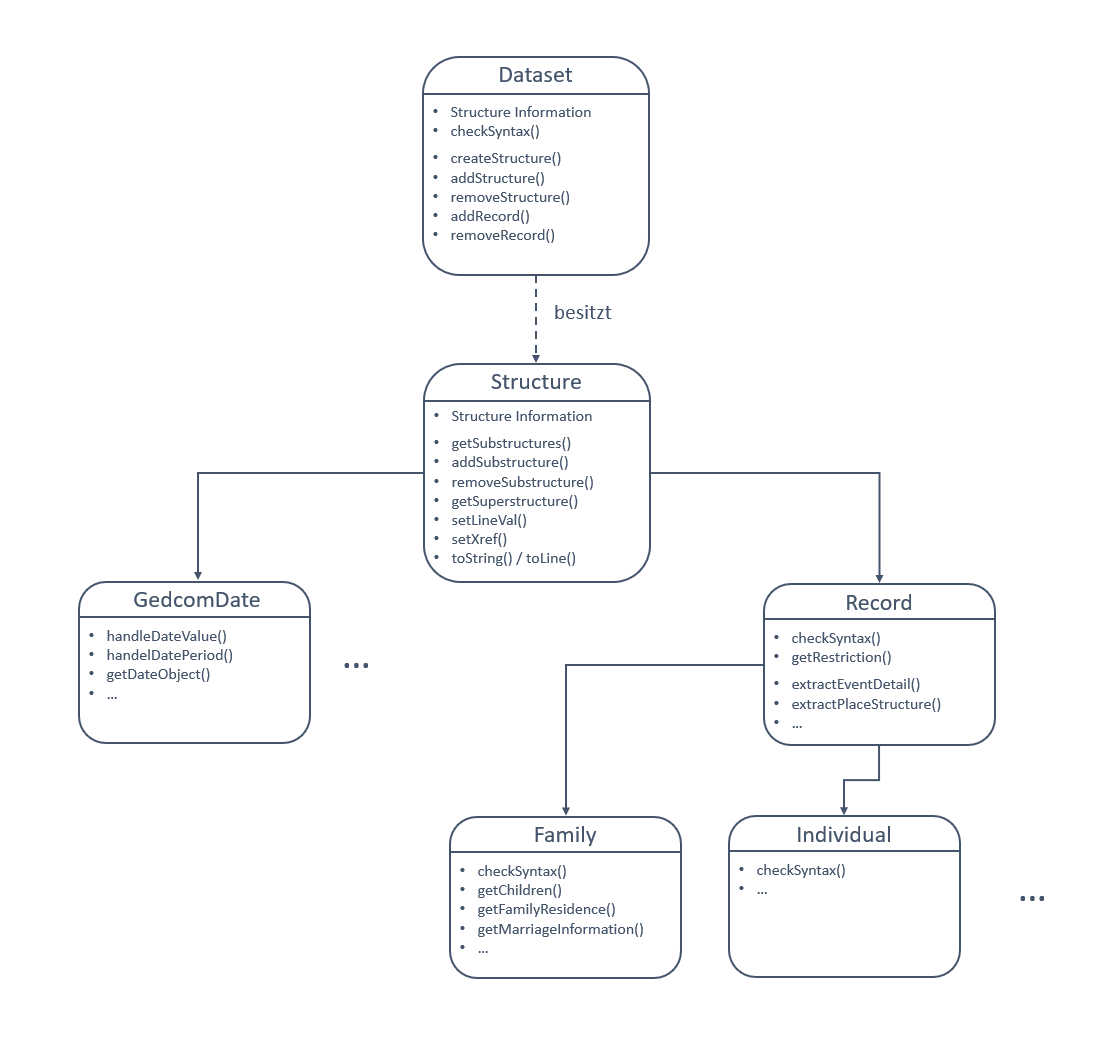
\includegraphics[width=1.0\textwidth]{images/konzept_structure.png}
	\caption{Gedcom Strukturen}
	\label{fig: Gedcom Strukturen}
\end{figure}

\subsection{Dataset}
\label{subsec: Konzept - Gedcom Strukturen - Dataset}
Die in Abschnitt \ref{subsec: Konzept - Gedcom Strukturen - Structure} beschriebenen Structures werden in einer \textit{Dataset} Datenstruktur zusammengefasst, die alle genealogischen Informationen einer Gedcom7 Datei enthält. Die Hauptaufgabe des Datasets besteht darin, Structures zu erstellen und zu verwalten. Wird eine Gedcom7 Datei mit korrekter Syntax mit dem in \ref{subsec: Konzept - Gedcom Grammatik - Nearley-Parser für Gedcom7} vorgestellten Nearley Parser eingelesen, extrahiert dieser alle Structure Informationen. Anschließend kann ein \textit{Dataset} erstellt werden, das all diese Informationen einliest, daraus Structures erstellt und die Zusammenhänge zwischen diesen Structures modelliert, sodass, eine Art Baumstruktur mit allen Records entsteht. Um ein Dataset mit neuen genealogischen Informationen anzureichern, sollen Methoden zum Hinzufügen bzw. zum Entfernen von Records bereitgestellt werden. Da das Hinzufügen bzw. Entfernen von Strukturen zu einer inkorrekten Gedcom7 Syntax führen kann, müssen Methoden zur Syntaxüberprüfung implementiert werden. Des Weiteren stellt das Dataset Metainformationen über eine Gedcom7 Datei zur Verfügung und sollte bestimmte Anforderungen überprüfen, die in der Gedcom7 Spezifikation angegeben werden. Beispiele hierfür sind, dass jede Gedcom7 Datei mit dem \textit{Byte-Order-Mark} beginnen sollte oder dass alle Structure, auf die über einen Cross-Reference-Identifier verwiesen wird, definiert seien müssen, bevor auf diese verwiesen wird. 
%========================================================================================
% SECTION: GEDCOM PARSER
%========================================================================================
\section{Gedcom Parser}
Die in diesem Kapitel vorgestellten Konzepte und Datenstrukturen werden alle im \textsc{Gedcom Parser} vereinigt, der die zentrale Instanz der Bibliothek \textit{gedcom7.js} darstellt. Abbildung \ref{fig: Sequenz Gedcom Parser} zeigt ein Sequenzdiagramm, das den allgemeinen Ablauf beim Einlesen einer Gedcom7 Datei mit dem \textsc{Gedcom Parser} zeigt.\\ 
Der \textsc{Gedcom Parser} ließt eine Gedcom7 Datei ein und konvertiert diese in eine Zeichenkette. Die Zeichenkette kann dann an einen Nearley Parser übergeben werden, der diese Line für Line ließt, die Syntax überprüft und dabei die Structure Informationen extrahiert. Ist die Syntax der Gedcom7 Datei korrekt, werden die gesammelten Structure Informationen an den Gedcom Parser zurückgegeben - anderenfalls wird das Einlesen mit einer Fehlermeldung beendet. Anschließend überprüft der Gedcom Parser die Kardinalität der eingelesenen Structures (beispielsweise darf nur eine \textit{HUSB}-Struktur pro Family Record enthalten sein).\footnote{Die Kardinalitätsüberprüfung wurde in den Gedcom Parser ausgelagert, da Nearley ein Streaming-Parser ist und somit zu keinem Zeitpunkt weiß, ob noch weitere Eingaben zu erwarten sind. Daher werden Konzepte wie Kardinalitätsüberprüfungen nicht von Nearley unterstützt. \cite{NearleyDoc}}. Sofern keine Fehler bei der Kardinalitätsüberprüfung gefunden werden, wird ein neues Dataset erstellt und die von Nearley extrahierten Structure Informationen an das Dataset übergeben. 


Das Dataset generiert den Header und den Trailer, der in jedem Dataset vorhanden sein muss und erstellt anschließend alle Structures auf Basis der Structure Informationen. Dazu wird jeder Eintrag der Structure Informationen auf den Structure Type untersucht (Record, Datatype Structure oder allgemeine Structure) und auf Basis dessen eine Structure mit allen Informationen erstellt. Diese Structure wird dann in das Dataset eingegliedert, indem die entsprechende Superstructure und alle Substructures zugewiesen werden. Sind alle Structures erstellt, wird überprüft, ob dass alle Cross-Reference-Identifier, auf die im Dataset verwiesen wird auch innerhalb des Datasets definiert sind. Ist dies der Fall, wird das Dataset zurückgegeben. Dieses Dataset kann dann wie in Abschnitt \ref{sec: Konzept - Gedcom Strukturen} beschrieben verändert und erweitert werden.

\begin{figure}[h]
	\centering
	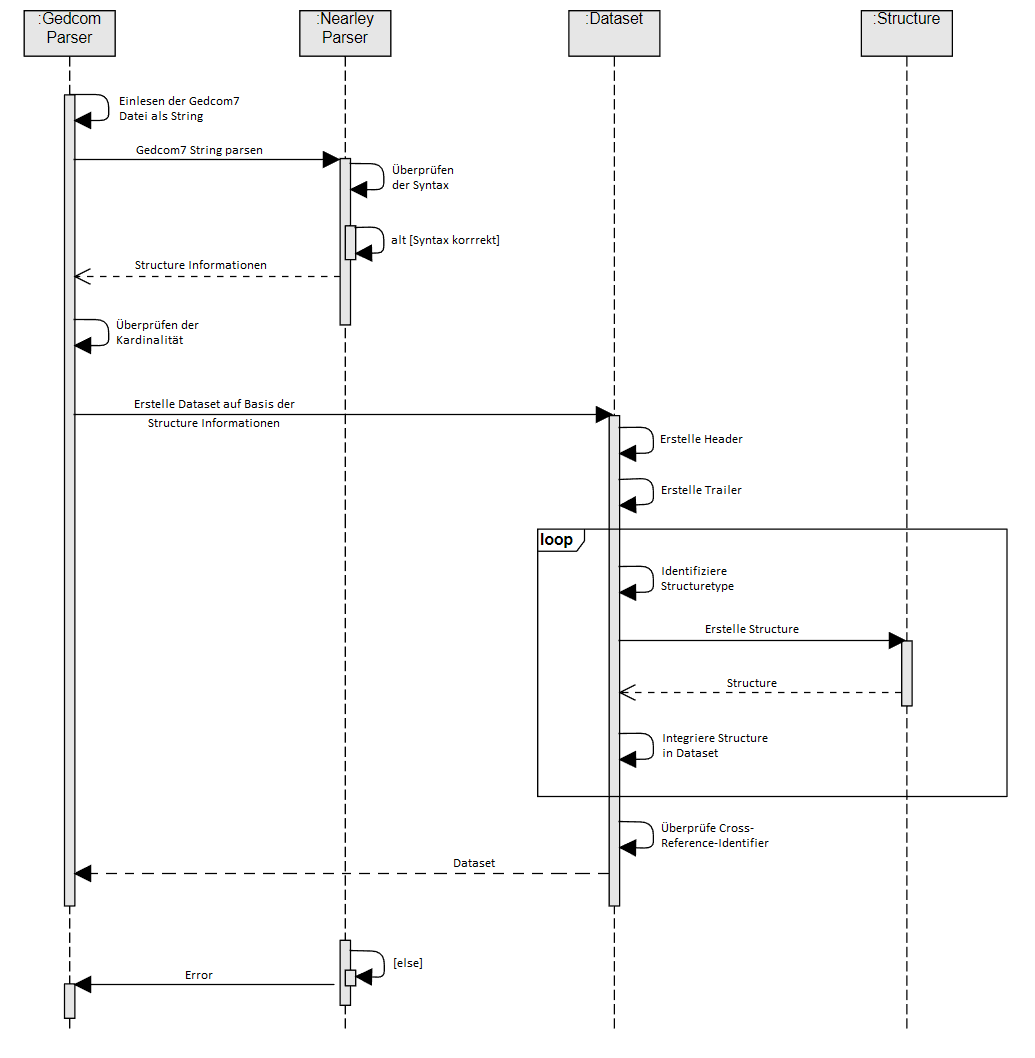
\includegraphics[width=1\textwidth]{images/konzept_sequenz.png}
	\caption{Ablauf Gedcom Parser}
	\label{fig: Sequenz Gedcom Parser}
\end{figure}
\label{sec: Konzept - Gedcom Parser}
